% This is text associated with the open textbook "Open Electromagnetics"
% See immediately below for author, date
% This work is licensed under the Creative Commons Attribution-ShareAlike 4.0 International License. (CC BY-SA 4.0) 
% To view a copy of the license, visit http://creativecommons.org/licenses/by-sa/4.0/

%ORB TITLE Capacitance of a Coaxial Structure
%ORB AUTHOR 0        # S.W. Ellingson, Virginia Tech (ellingson@vt.edu)
%ORB DATE 20180806   # yyyymmdd
%ORB ABSTRACT Capacitance of a Coaxial Transmission Line

\label{m0113_Capacitance_of_Coaxial_Line} % <-- Must match name of this file and module directory name.  Don't mess with this!

Let us now determine the capacitance of coaxially-arranged conductors, shown in Figure~\ref{m0113_fCapCoax}.
Among other applications, this information is useful in the analysis of voltage and current waves on coaxial transmission line, as addressed in Sections~\ref{m0029_Lumped-Element_Model} and \ref{m0143_Coaxial_Line}.

For our present purposes, we may model the structure as consisting of two concentric perfectly-conducting cylinders of radii $a$ and $b$, separated by an ideal dielectric having permittivity $\epsilon_s$.
We place the $+z$ axis along the common axis of the concentric cylinders so that the cylinders may be described as constant-coordinate surfaces $\rho=a$ and $\rho=b$.
%
\begin{figure}[b!]
\begin{center}
\pdftooltip{{  % note double braces
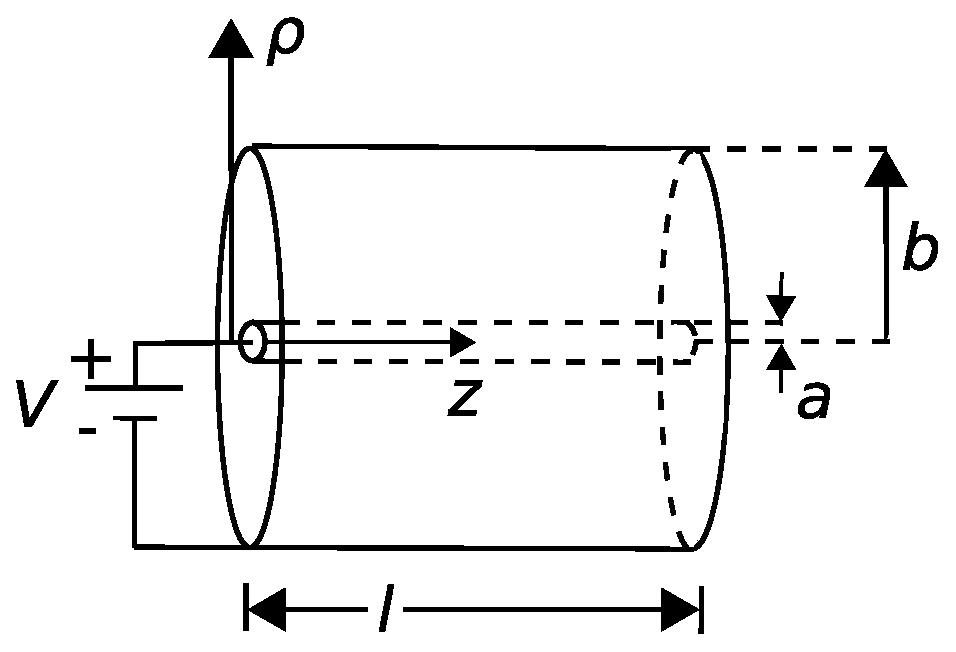
\includegraphics[width=2.5in]{modules/m0113_fCapCoax.eps}
% https://commons.wikimedia.org/wiki/File:M0113_fCapCoax.svg
}}{A three dimensional cylinder with length l and radius b lies on its side with a narrow concentric cylinder through the middle with similar length and radius a. A battery is attached to the interior cylinder by its positive side, and the negative side attached to the exterior cylinder. The vector z is shown pointing to the right from the left edge of the interior cylinder. A vector rho extends up from the point of connection perpendicular to z.}
\end{center} 
\centerline{\scriptsize 
\copyright~\hyperref[m0113_fCapCoax_Credit]{K.\ Kikkeri} 
\href{https://creativecommons.org/licenses/by-sa/4.0/}{CC BY~SA 4.0} 
} 
\caption{
\label{m0113_fCapCoax}
Determining the capacitance of a coaxial structure.
}
\end{figure}

In this section, we shall find the capacitance by assuming a total charge $Q_+$ on the inner conductor and integrating over the associated electric field to obtain the voltage between the conductors.  Then, capacitance is computed as the ratio of the assumed charge to the resulting potential difference.
This strategy is the same as that employed in Section~\ref{m0070_Parallel_Plate_Capacitor_Capacitance_from_Charge} for the parallel plate capacitor, so it may be useful to review that section before attempting this derivation.

The first step is to find the electric field inside the structure.
This is relatively simple if we assume that the structure has infinite length (i.e., $l\to\infty$), since then there are no fringing fields and the internal field will be utterly constant with respect to $z$.
In the central region of a finite-length capacitor, however, the field is not much different from the field that exists in the case of infinite length, and if the energy storage in fringing fields is negligible compared to the energy storage in this central region then there is no harm in assuming the internal field is constant with $z$. 
Alternatively, we may think of the length $l$ as pertaining to one short section of a much longer structure and thereby obtain the capacitance \emph{per length} as opposed to the total capacitance.
Note that the latter is exactly what we need for the transmission line lumped-element equivalent circuit model (Section~\ref{m0029_Lumped-Element_Model}). 

To determine the capacitance, we invoke the definition (Section~\ref{m0112_Capacitance}):
%
\begin{equation}
C \triangleq \frac{Q_+}{V}
\label{m0113_eCapDef}
\end{equation}
%
where $Q_+$ is the charge on the positively-charged conductor and $V$ is the potential measured from the negative conductor to the positive conductor.
The charge on the inner conductor is uniformly-distributed with density 
%
\begin{equation}
\rho_l = \frac{Q_+}{l}
\end{equation}
%
which has units of C/m.
Now we will determine the electric field intensity ${\bf E}$, integrate ${\bf E}$ over a path between conductors to get $V$, and then apply Equation~\ref{m0113_eCapDef} to obtain the capacitance.

The electric field intensity for this scenario was determined in Section~\ref{m0149_E_due_to_Inf_Line_Charge}, ``Electric Field Due to an Infinite Line Charge using Gauss' Law,'' where we found
%
\begin{equation}
{\bf E} = \hat{\rho} \frac{\rho_l}{2\pi \epsilon_s \rho}
\end{equation}
%
The reader should note that in that section we were considering merely a line of charge; not a coaxial structure.
So, on what basis do we claim the field is the same?
This is a consequence of Gauss' Law (Section~\ref{m0014_Gauss_Law_Integral_Form})
%
\begin{equation}
\oint_{\mathcal S} {\bf D}\cdot d{\bf s} = Q_{encl}
\end{equation}
%
which we used in Section~\ref{m0149_E_due_to_Inf_Line_Charge} to find the field.
If in this new problem we specify the same cylindrical surface $\mathcal{S}$ with radius $\rho<b$, then the enclosed charge is the same.
Furthermore, the presence of the outer conductor does not change the radial symmetry of the problem, and nothing else remains that can change the outcome.
This is worth noting for future reference:
%
%ORB HIGHLIGHT
\begin{mdframed}[backgroundcolor=yellow!20,nobreak=true] 
The electric field inside a coaxial structure comprised of concentric conductors and having uniform charge density on the inner conductor is identical to the electric field of a line charge in free space having the same charge density.
\end{mdframed}

Next, we get $V$ using (Section~\ref{m0061_Force_Energy_and_Potential_Difference})
%
\begin{equation}
V = -\int_{\mathcal C}{ {\bf E} \cdot d{\bf l} }
\end{equation}
%
where $\mathcal{C}$ is any path from the negatively-charged outer conductor to the positively-charged inner conductor.
Since this can be \emph{any} such path (Section~\ref{m0062_Independence_of_Path}), we may as well choose the simplest one.
This path is the one that traverses a radial of constant $\phi$ and $z$.
Thus: 
%
\begin{flalign}
V &= -\int_{\rho=b}^a{ \left( \hat{\bf \rho} \frac{\rho_l}{2\pi \epsilon_s \rho} \right) \cdot \left(\hat{\bf \rho}d\rho\right) }  \nonumber \\
  &= - \frac{\rho_l}{2\pi \epsilon_s} \int_{\rho=b}^a{ \frac{d\rho}{\rho}  }  \nonumber \\
  &= + \frac{\rho_l}{2\pi \epsilon_s} \int_{\rho=a}^b{ \frac{d\rho}{\rho}  }  \nonumber \\
  &= + \frac{\rho_l}{2\pi \epsilon_s} \ln\left(\frac{b}{a}\right)
\end{flalign} 

Wrapping up:
%
\begin{equation}
C \triangleq \frac{Q_+}{V} = \frac{\rho_l l}{ \left( \rho_l / 2\pi \epsilon_s \right) \ln\left(b/a\right) }
\end{equation}
%
Note that factors of $\rho_l$ in the numerator and denominator cancel out, leaving:
%
\begin{equation}
\boxed{
C = \frac{2\pi \epsilon_s l}{\ln\left(b/a\right)}   
}
\end{equation}
%
Note that this expression is dimensionally correct, having units of F. 
Also note that the expression depends only on materials (through $\epsilon_s$) and geometry (through $l$, $a$, and $b$).
The expression does \emph{not} depend on charge or voltage, which would imply non-linear behavior.

To make the connection back to lumped-element transmission line model parameters (Sections~\ref{m0029_Lumped-Element_Model} and \ref{m0143_Coaxial_Line}), we simply divide by $l$ to get the per-unit length parameter:
%
\begin{equation}
\boxed{
C' = \frac{2\pi \epsilon_s}{\ln\left(b/a\right)}   
}
\label{m0113_eCp}
\end{equation}

\index{transmission line!coaxial|(}
%ORB EXAMPLE
~\\ \begin{example} 
\begin{mdframed}[backgroundcolor=brown!20,linecolor=brown!20]\raggedright
Capacitance of RG-59 
\index{RG-59}
coaxial cable.
\\~\\
RG-59 coaxial cable consists of an inner conductor having radius $0.292$~mm, an outer conductor having radius $1.855$~mm, and a polyethylene spacing material having relative permittivity 2.25.
Estimate the capacitance per length of RG-59.

{\bf Solution.} 
From the problem statement, 
$a=0.292$~mm, 
$b=1.855$~mm, 
and $\epsilon_s = 2.25\epsilon_0$.
Using Equation~\ref{m0113_eCp} we find $C'=67.7$~pF/m.
\end{mdframed}\end{example}

\index{transmission line!coaxial|)}
